\documentclass[11pt, a4paper]{article}
\usepackage{amsmath, amsthm, amssymb, calrsfs, wasysym, verbatim, bbm, color, graphics, geometry}
\usepackage[utf8]{inputenc} % comment when using lualatex
\usepackage[italian]{babel} % lingua e a-capo-sillabato
\usepackage{fullpage}
\usepackage{graphicx}
%\usepackage[hidelinks]{hyperref,xcolor} % link di pagina
\usepackage[bottom]{footmisc} % note appiccicate al fondo della pagina
\usepackage{float} % per posizionamento immagini

\geometry{tmargin=.75in, bmargin=.75in, lmargin=.75in, rmargin = .75in}  

\newcommand{\R}{\mathbb{R}}
\newcommand{\C}{\mathbb{C}}
\newcommand{\Z}{\mathbb{Z}}
\newcommand{\N}{\mathbb{N}}
\newcommand{\Q}{\mathbb{Q}}
\newcommand{\Cdot}{\boldsymbol{\cdot}}

\newtheorem{thm}{Theorem}
\newtheorem{defn}{Definition}
\newtheorem{conv}{Convention}
\newtheorem{rem}{Remark}
\newtheorem{lem}{Lemma}
\newtheorem{cor}{Corollary}



\definecolor{dkgreen}{rgb}{0,0.6,0}
\definecolor{gray}{rgb}{0.5,0.5,0.5}
\definecolor{mauve}{rgb}{0.58,0,0.82}


\title{Network Infrastructures }
\author{Raffaele Castagna}

\date{Academic Year 2025-2026}

\begin{document}

\maketitle
\tableofcontents
\newpage
\section{Network functional areas}
An \textbf{Access network} is part of a communications network which connect subscribers to their service provider, to actually connect them historically ISPs have used copper lines which also carried phone signals, but they have now heavily invested into optical fiber cables.\\\\
The \textbf{Core network} is a backbone network, it has always used fiber optic cables and it is constitued by the optical backbone, we could say that the internet is a giant core network, since it consists of many service providers that run their own core networks, which are interconnected.\\\\
The \textbf{Edge network} is located between acess and core, it used to decide which path the packets should take using MPLS (multiprotocol Label Switching), It is used to decide the service the user wants to use, but it's also used to run
services that in the past where run in the cloud, they need to run closer to the
user, for example. The closer they run, the least the delay.
So the edge is fundamental to distinguish the kind of service we use, but also
because it hosts computing servers (known as edge computing)\\\\
We have different types of accesses:
\begin{itemize}
    \item \textbf{Wired access}, high reliability, high speed, low latency
    \item \textbf{Wireless access}, mobile, flexibile and easy to setup.
    \item \textbf{Satellite Access} Wide coverage, suitable for remote areas.
    \item \textbf{Fiber Optic Access} uses fiber optics (so costly) but high speed and low latency.
    \item \textbf{DSL Access} Widespread and cost effective
    \item \textbf{Cable Access} uses coaxial cables, high speed and widely available, suitable for TV
\end{itemize}
and many more...\\\\
\subsection{FTTX}
With fiber becoming widespread we have what we call FTTX (fiber to the X) where X can be:
\begin{itemize}
    \item \textbf{FTTH} Fiber to the home
    \item \textbf{FTTB} Fiber to the building
    \item \textbf{FTTC} Fiber to the curb
    \item \textbf{FTTN} Fiber to the node
    \item \textbf{FTTP} Fiber to the premises
    \item \textbf{FTTD} Fiber to the desk
    \item \textbf{FTTU} Fiber to the user
    \item \textbf{FTTO} Fiber to the office
    \item \textbf{FTTZ} Fiber to the zone
\end{itemize}
In fttx we have multiple elements, the OLT (optical line terminal) the ONU (Optical Network Unit) , the ONT (Optical Network Termination) and the ODN, Optical Distribution Network.
\begin{center}
    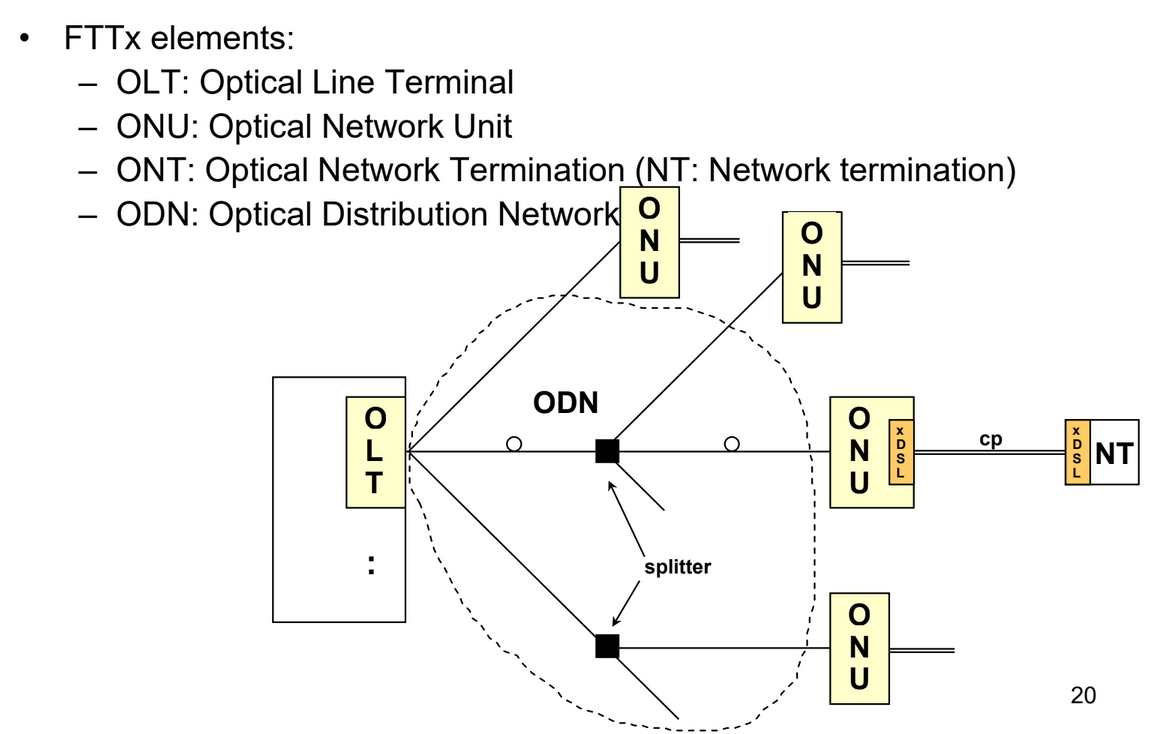
\includegraphics[scale=0.5]{img/AccessNetworks/FTTX/reference.png}
\end{center}
These can be used in multiple ways to create an infrastructure, one example is AON (Active Optical Network), where the loops represent the fiber. This topology is not used as the cost from local exchange to user is pretty high, as fiber has a high labor cost. 70€/m \\
A possible solution is a single fiber to a single element, called active element which shortens the path you need to dig. The active node receives light and then converts it into electricity and then converts it into another light signal.
\begin{center}
    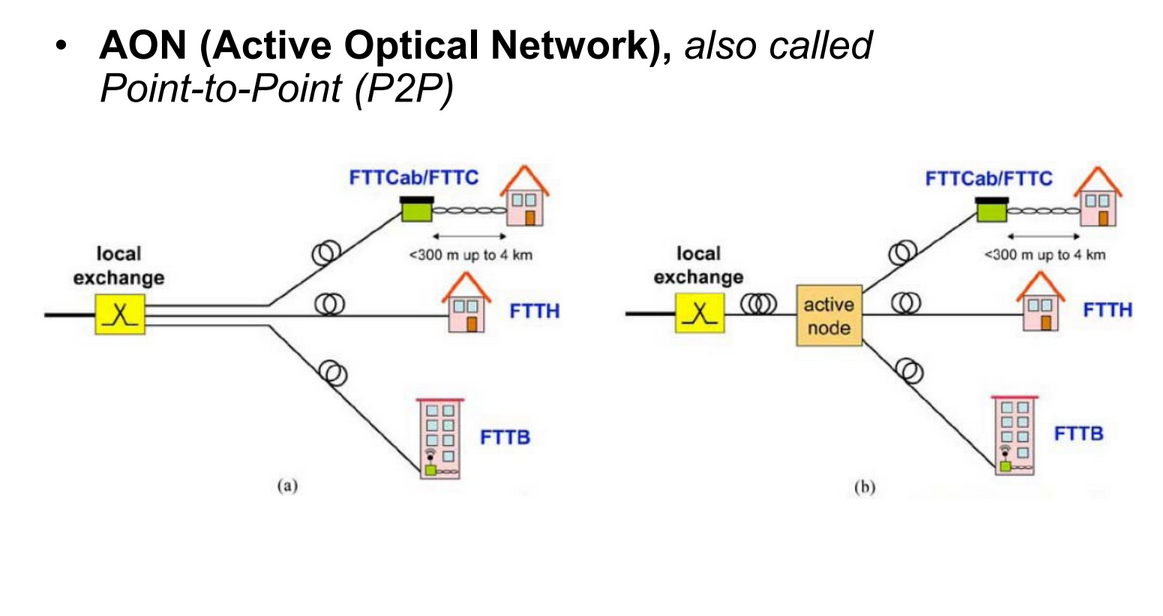
\includegraphics[scale=0.5]{img/AccessNetworks/FTTX/AON.png}
\end{center}
In the fiber domain we have a more favorable solution, the PON (Passive optical network),where instead of an active node we have an optical power splitter/combiner which does not use electricity, in this case when we split, the same signal arrives to everyone, but only the ONU/ONT that recognizes its address will process the signal, the others will discard it. This is a more cost effective solution as we don't need electricity, but the signal weakens as we split it, so we need to be careful about how many splits we do.
\begin{center}
    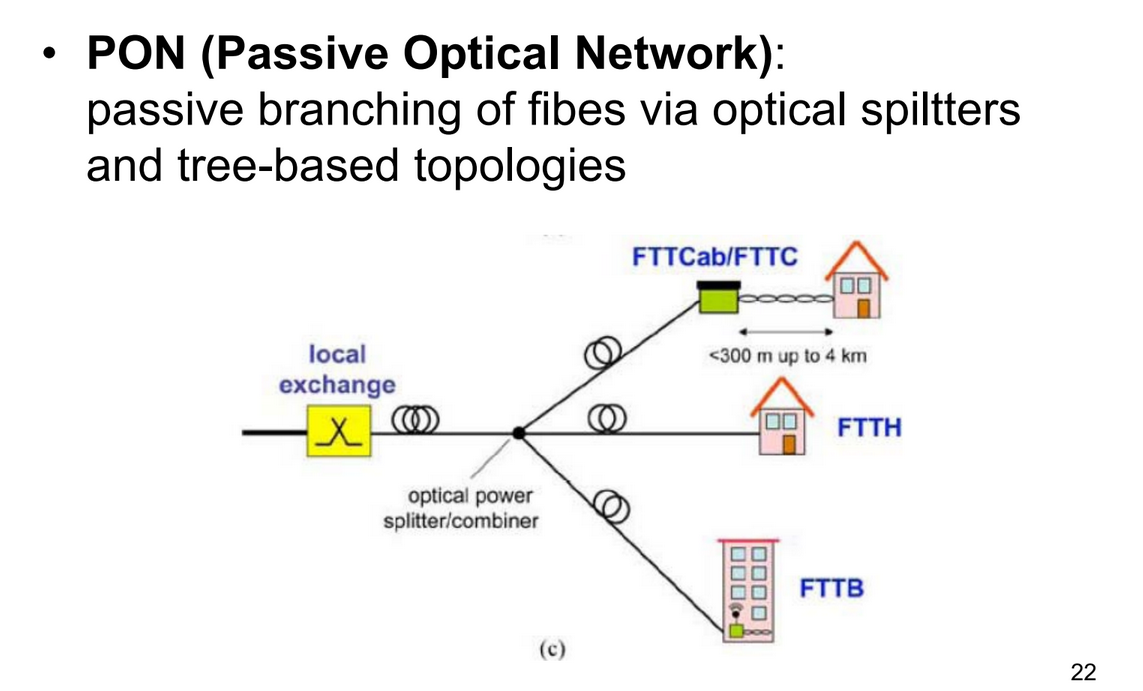
\includegraphics[scale=0.5]{img/AccessNetworks/FTTX/PON.png}
\end{center}
We also have fiber to the exchange, where fiber terminates to the central office and is then connected via copper (e.g. ADSL) (VDSL is very high speed digital subscriber line)
\begin{center}
    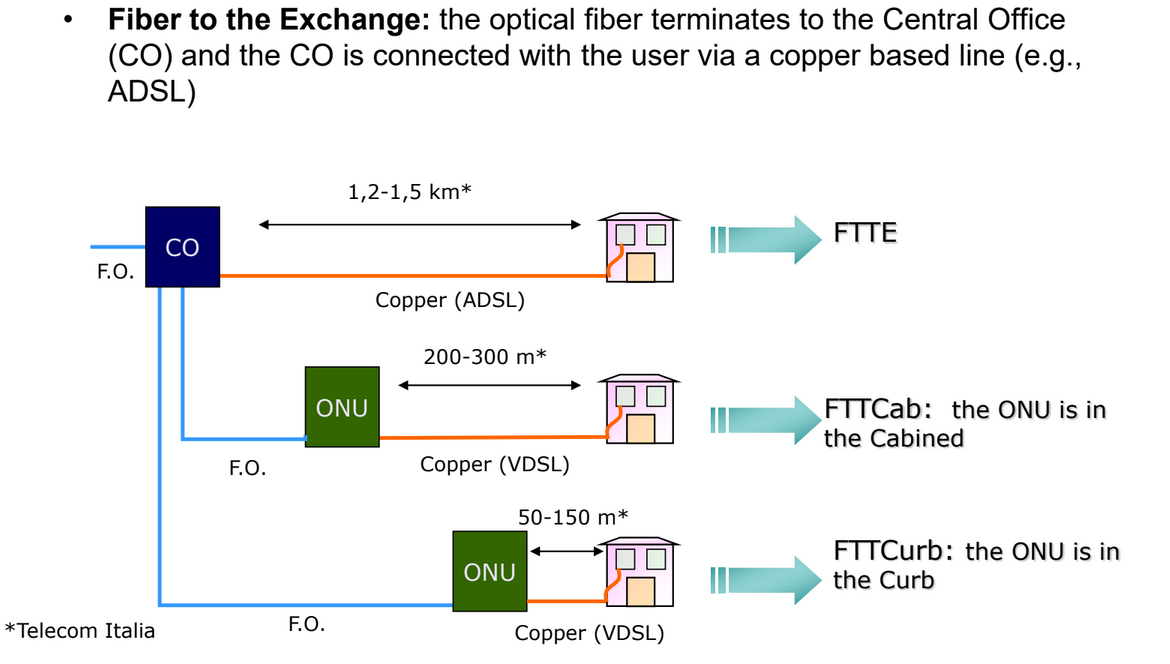
\includegraphics[scale=0.5]{img/AccessNetworks/FTTX/FTTX.png}
\end{center}
We also have FTTC which is fiber to the curb, or more commonly fiber to the cabinet, where the fiber terminates near the building, and then the last mile is done via copper (e.g. VDSL).\\
After that we have the various FTTP/FTTB/FTTH.
\begin{center}
    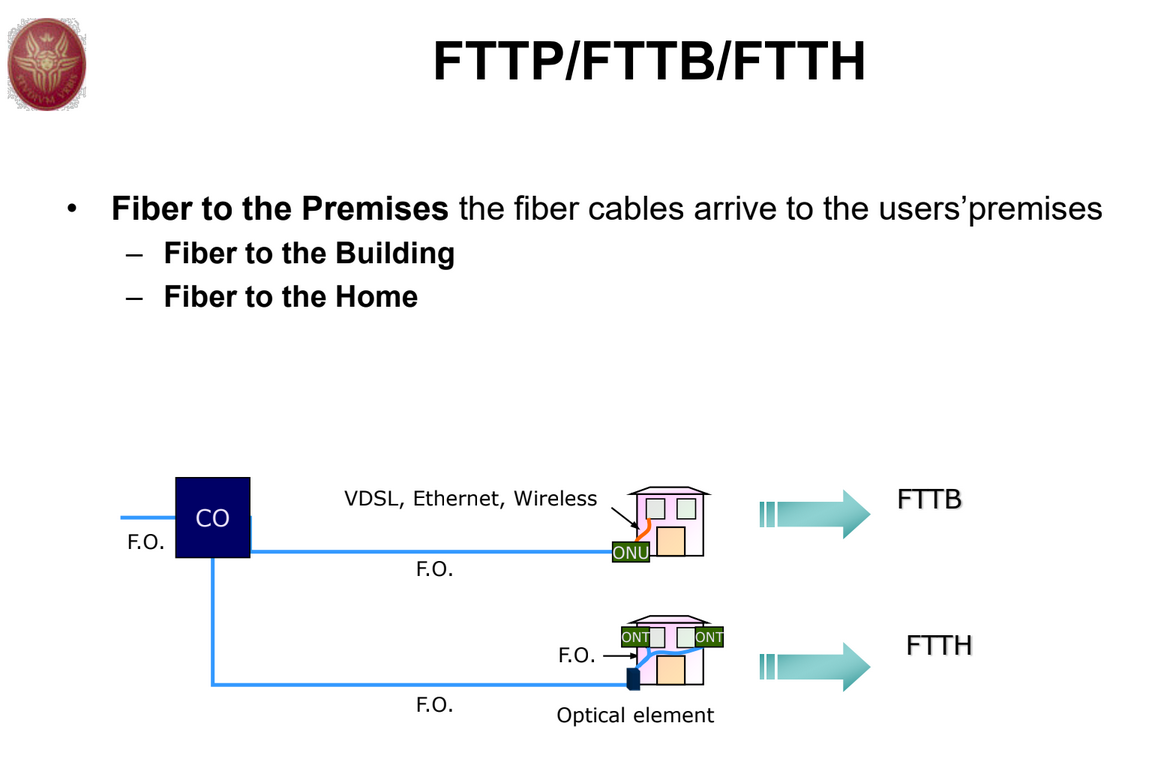
\includegraphics[scale=0.5]{img/AccessNetworks/FTTX/FTTP.png}
\end{center}
\subsection{Wireless Access Networks}
Sometimes it isn't economical to dig/ it isn't worth the trouble, so we use wireless access networks, which are very complicated.
Areas are divided into cells, in each cell we find an antenna (base station), antennas are also connected to the backhole (in the past made with copper).\\
\textit{Note:}Availability means localizing the user and then managing the information regarding the movement of the user
\begin{center}
    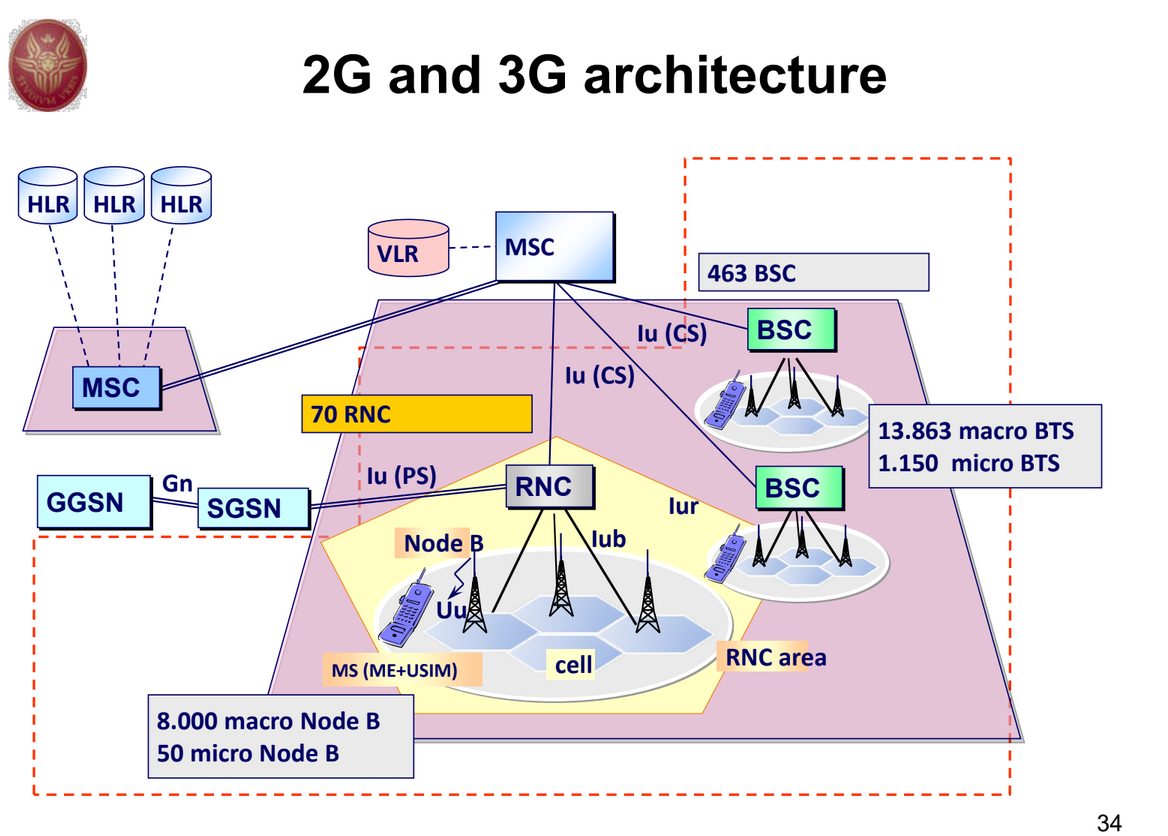
\includegraphics[scale=0.5]{img/AccessNetworks/Wireless/2G.png}
\end{center}
We also have 5g networks, where we have the User equipment, the antenna is called the gNodeB, the access and mobility management function AMF, session Management Function SMF, and User Plane Function UPF, the User Plane is both hardware and software and the Control Plane is software, the antenna is hardware ofc.
\begin{center}
    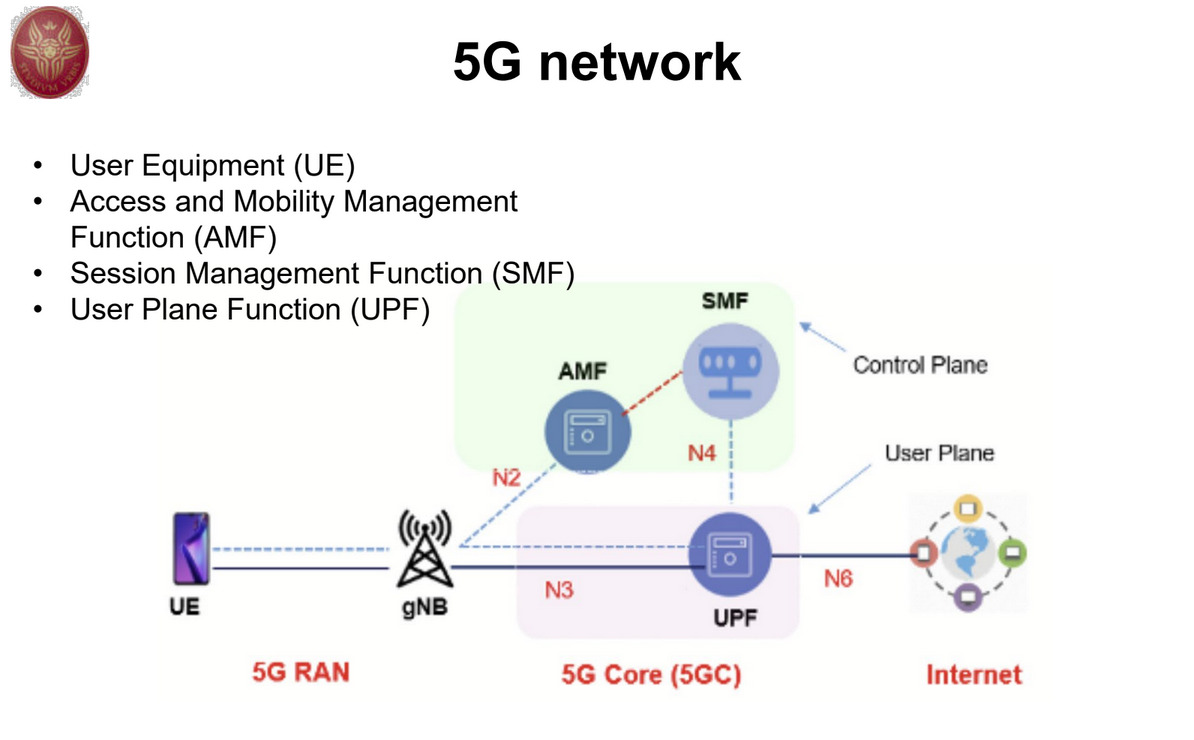
\includegraphics[scale=0.5]{img/AccessNetworks/Wireless/5G.png}
\end{center}
\subsection{Satellite Access Networks}
Around ~500-2000 km above earth with a short orbital period, it gives low latency communications, therefore it requires a lot of satellites, they utilize the Ku and Ka Band.\\
So the advantages are low latency, high bandwidth potential and it gives us global coverage, but the challenges we face are the large amount of satellites needed, there's a high deployment and maintenance costs, along with space debris and a short satellite lifespan.\\
\subsection{XDSL}
Dsl stands for digital subscriber line (subscriber of a contract), it has many different standards:
\begin{itemize}
    \item ISDL 
    \item HDSL
    \item SDSL
    \item ADSL
    \item ADSL lite
    \item RADSL
    \item VDSLV
    \item VDSL2
\end{itemize}
In the first iterations the telephone distribution network featured a twisted pair for each user, connecting them to the
CO. Bundles of twisted pairs from various users converged at a cabinet and were aggregated to
the CO. Early DSL iterations like ISDN (the first DSL) doubled the connections by aggregating
two twisted pairs to enable one channel for voice and another for data. However, However, the
fact that the bandwidth used by the user for data transmission is the same as that used by voice
traffic (4 kHz) soon became a bottleneck.
\begin{center}
    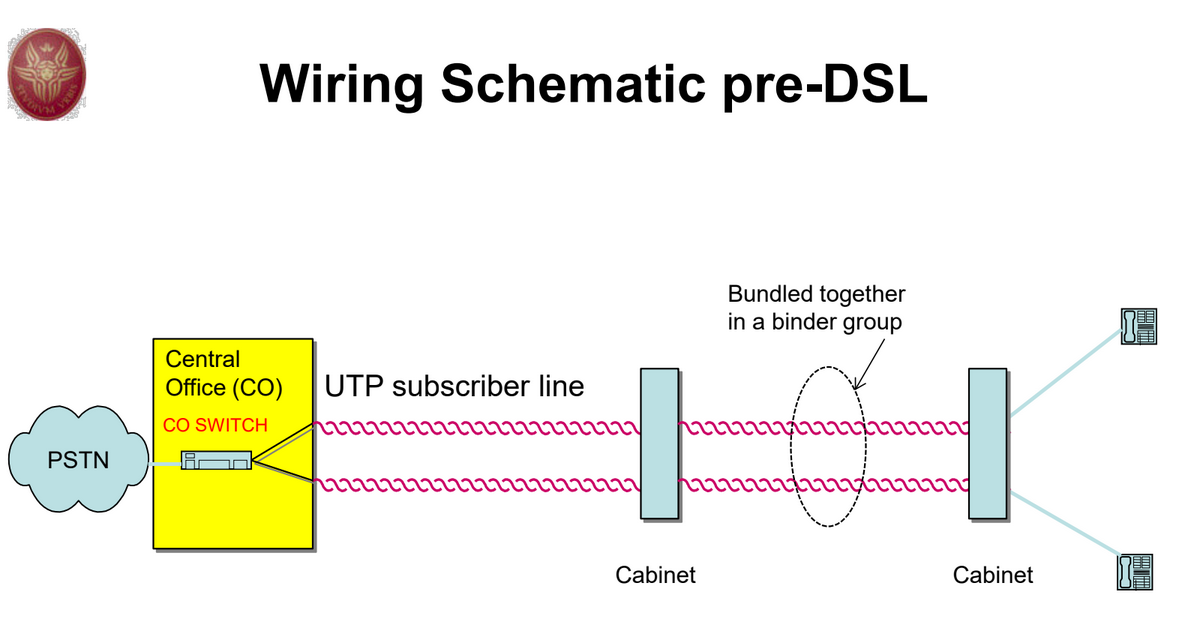
\includegraphics[scale=0.5]{img/AccessNetworks/XDSL/Schematic.png}
\end{center}
Analog modems represented a foundational method for delivering data services via the local
telephone network. These devices were capable of transmitting data at speeds of 56 Kbps,
effectively converting digital data into analog signals suitable for transmission over standard
telephone lines. The same connection could alternate between voice and data transmission,
though not simultaneously.
To achieve data transfer, voice modems utilized the voice frequency band, essentially
simulating a phone call to relay information. Once transmitted, the central office (C.O.) detected
and processed this signal as data. Each data session incurred charges equivalent to a standard
phone call, making prolonged usage financially burdensome.
\begin{center}
    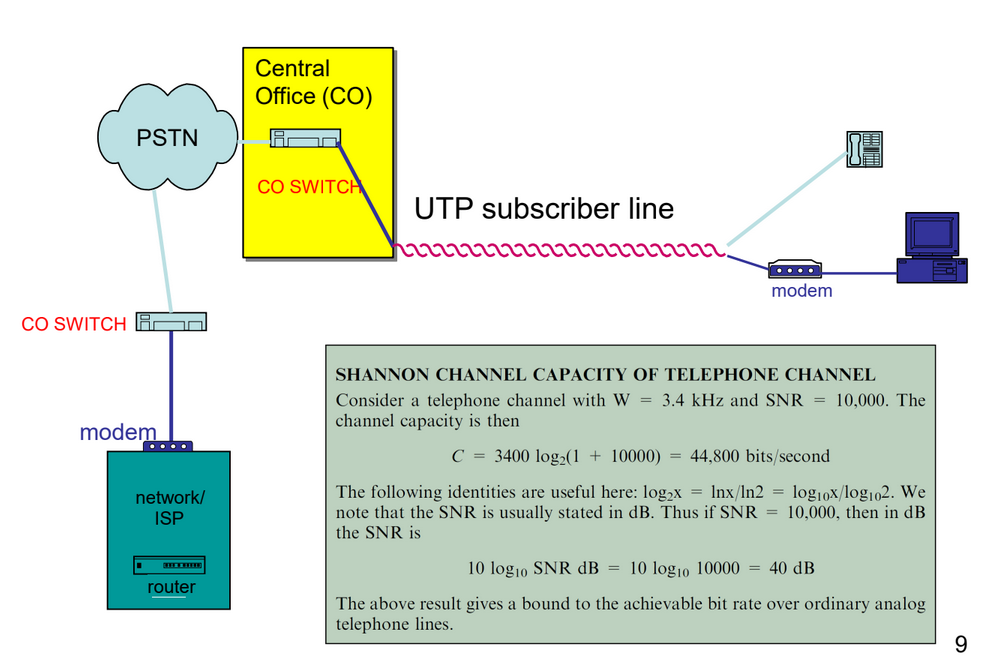
\includegraphics[scale=0.5]{img/AccessNetworks/XDSL/Shannon.png}
\end{center}
Even after we stopped using the 4 khZ band we still had limitations that had to do with the space inside the C.O. and the fact that the performance of copper degraded with long cables.\\
\subsection{ADSL}
ADSL (Asymmetric Digital Subscriber Line) is a type of DSL technology that provides high-speed internet access over traditional copper telephone lines. It is called "asymmetric" because it offers different speeds for downloading and uploading data, with download speeds typically being much higher than upload speeds. This asymmetry is designed to accommodate the typical usage patterns of internet users, who often download more data than they upload.\\\\
ADSL utilizes higher frequency bands on the copper line, but this introduces more interference (a signal overlaps in time and frequency) and attenuation, to counteract this ADSL uses multiple such as frequency division and eco cancellation, in frequency division we divide the frequency band into two parts, one for upstream data and one for downstream data. In echo cancellation we use the same frequency band for both upstream and downstream data, but we use a technique called echo cancellation to separate the two signals.\\
\begin{center}
    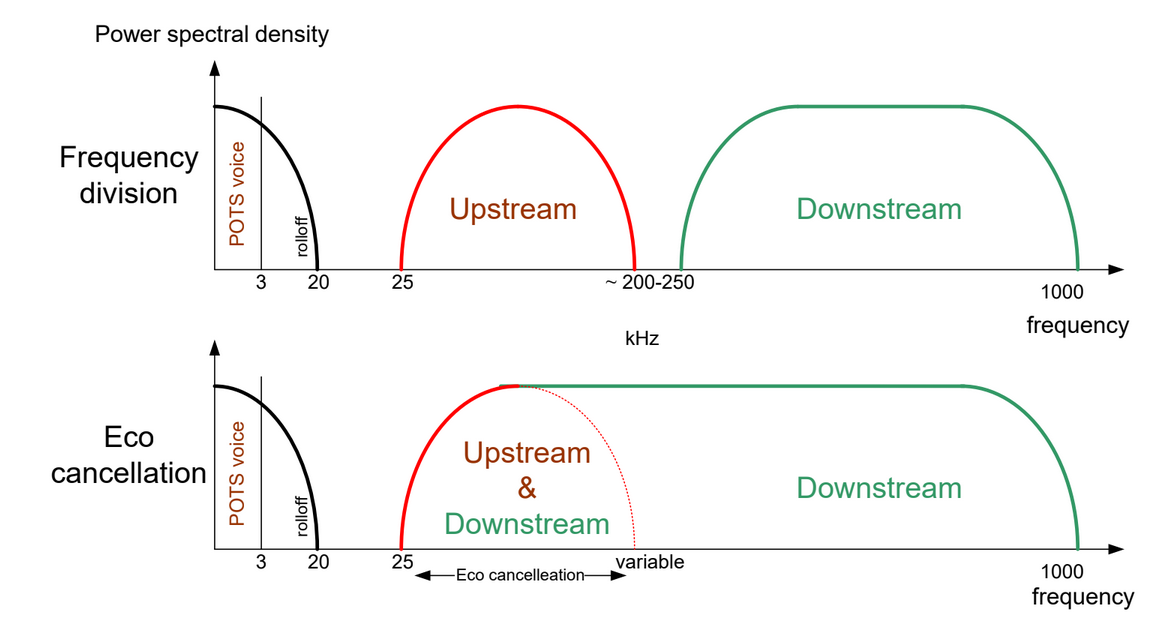
\includegraphics[scale=0.5]{img/AccessNetworks/XDSL/Frequency.png}
\end{center}
We can formalize this via FEXT (far end cross-talk), the cross talk between transmitter and a receiver placed on opposite sides of the cable. You can measure interference at the receiver side.
\begin{center}
    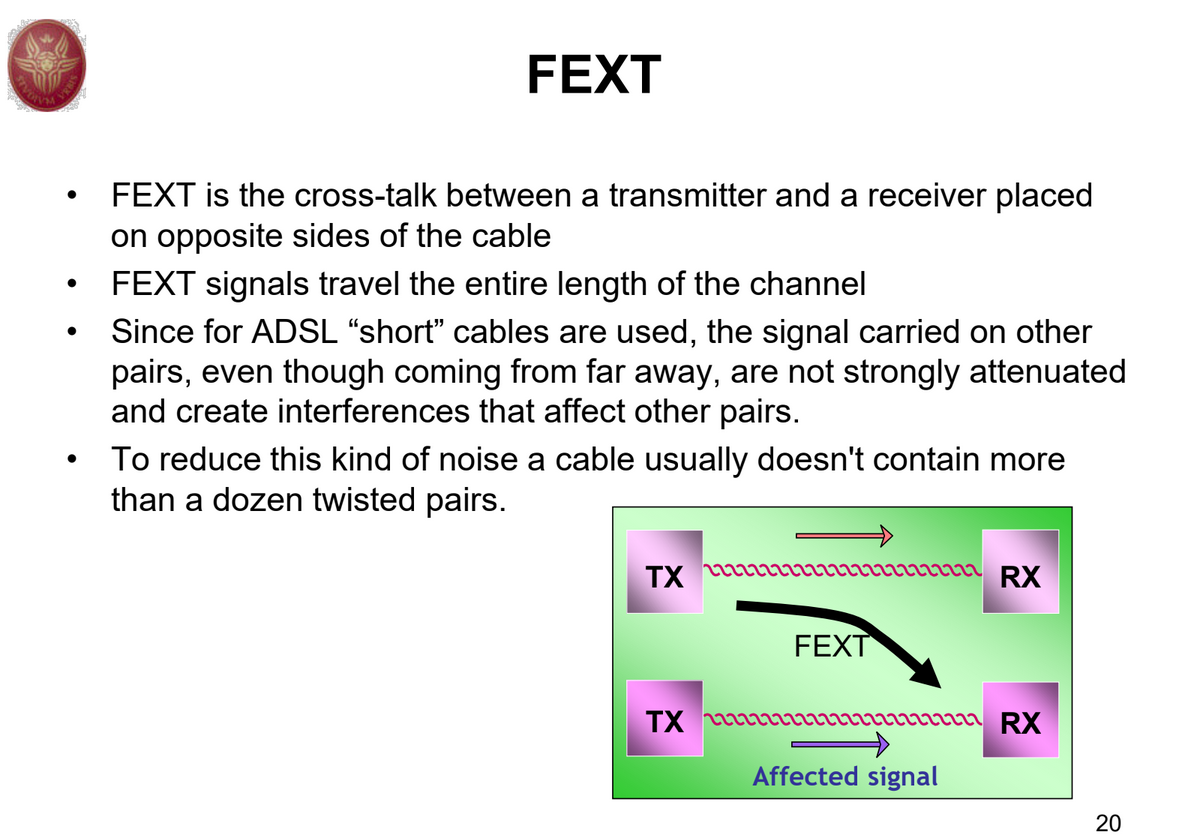
\includegraphics[scale=0.5]{img/AccessNetworks/XDSL/FEXT.png}
\end{center}
We also have NEXT where the receiver is near the transmitter and we have the same problem.
\begin{center}
    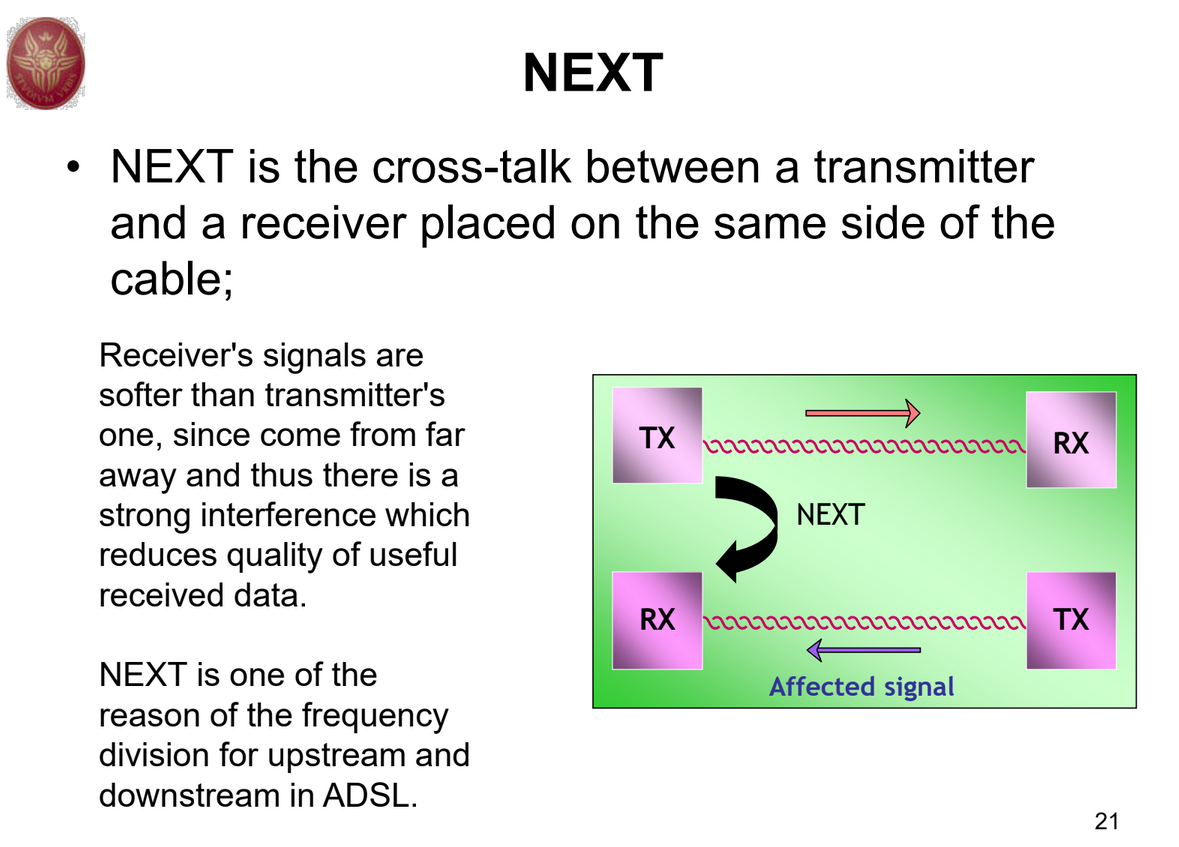
\includegraphics[scale=0.5]{img/AccessNetworks/XDSL/NEXT.png}
\end{center}
If we were using the same type of connection (down) we may have interference, but remember that interference in calculated at the receiver side, plus we have interference only if the cables are near (centimeters), this may also happen if we use echo cancellation and occupy part of the upstream.
By transmitting downstream data within the upstream band, the C.O. can apply echo
cancellation.\\
The C.O. knows its downstream transmissions and the upstream data it receives, enabling
it to remove interference caused by overlapping flows.\\
This technique effectively increases the downstream data rate by omitting the upstream
portion when necessary.\\\\
When we have both a telephone and ADSL line, we may have problems when dialing a phone call, to forego this problem we installed filters to separate the communications.\\\\
We also may have signal attenuation, which if we know it and it is constant, we can amplify the signal. The rule is that if you have a short bandwidth then the attenuation is constant, if it isn't short, it isn't costant, to solve this problem you split the bandwidth into different channels with low bandwidth, but since we can transmit simultaneously then we have around the same speed.
\end{document}